\documentclass[a4paper, 11pt]{article}

\usepackage[utf8]{inputenc}
\usepackage[frenchb]{babel}
\usepackage[T1]{fontenc}
\usepackage{textcomp}
\usepackage{amsmath,amssymb}
\usepackage{lmodern}
\usepackage[a4paper]{geometry}
\usepackage{graphicx}
\usepackage{xcolor}
\usepackage{microtype}
\usepackage{listings}
\usepackage{hyperref}

\title{Aide à la décision}
\author{Dragibus}
\date{}

\begin{document}
\maketitle
\tableofcontents
\newpage

\section{Introduction}
Cette étude se déroulera en trois parties. Dans la première nous considèrerons
le nombre de produits de chaque type à produire pour optimiser les critères
retenus par chaque cadre de l'entreprise ADécision. La deuxième partie
comprendra une analyse de tous les critères considérés dans la première partie
et la recherche d'une solution de compromis satisfaisant chacun d'entre-eux. La
dernière partie consistera en l d'une solution finale parmis celles
proposées précédemment.

\subsection{Définition}
Nous définissons ici les notations que nous utiliserons dans la suite de ce
rapport et exprimmons certaines notions sous forme de fonctions mathématiques.
\\
Soit $E_M = \left\{1, 2, 3, 4, 5, 6, 7\right\} $ l'ensemble des machines. \\
Soit $E_{MP} = \left\{MP1, MP2, MP3\right\} $ l'ensemble des matières premières. \\
Soit $E_P = \left\{A, B, C, D, E, F\right\} $ l'ensemble des produits. \\
Soit $B$ le bénéfice de l'entreprise. \\
Soit $TTH$ le temps de travail hebdomadaire. \\
Soit $X(i)$ le nombre de produit $i\in E_P$ fait. \\
Soit $X = \left\{X(1), X(2), X(3), X(4), X(5), X(6), X(7)\right\}$ le vecteur
définissant les quantités de chaque produit à fabriquer.\\
Soit $S(p)$ la quantité en stock de la matière première $p\in E_{MP}$. \\
Soit $TM(m)$ le temps d'utilisation de la machine $m\in E_M$.\\
Soit $G(i)$ le gain engendré par le produit $i$. \\
Soit $V(i)$ le prix de vente du produit $i$. \\
Soit $P(i)$ la perte engendrée par le produit $i$. \\
Soit $Q(i, p)$ la quantité de matière $p$ nécessaire pour le produit $i$. \\
Soit $A(p)$ le prix d'achat de la matière $p$. \\
Soit $C(m)$ le cout de la machine $m$. \\
Soit $T(i, m)$ le temps d'usinage de la machine $m$ pour le produit $i$. \\

$$
\begin{array}{r l}
    G(i) =  & V(i)\cdot X(i) \\
    P(i) =  & X(i)\left(\sum_{p\in E_{MP}} A(p)Q(i, p)+ \sum_{m\in E_M} C(m)T(i, m)\right) \\
    B =     & \sum_{i\in E_P} G(i) - P(i) \\
    TM(m) = & \sum_{i\in E_P} X(i)T(i, m) \\
    TTH =   & \sum_{m\in E_M} TM(m) \\
    S(p) =  & \sum_{i\in E_P} X(i)Q(i, p) \\
\end{array}
$$

\subsection{Ensemble des contraintes}
Cette section exprime sous forme mathématique les différentes contraintes
inhérentes au fonctionnement de l'entreprise.

$$
\begin{array}{r l}
    \forall i\in E_P, & X(i) > 0 \\
    \forall m\in E_M, & TM(m) \in [0, 4800\mbox{min}] \\
                      & TTH \in [0, 4800\mbox{min}] \\
                      & B > 0 \\
                      & S(MP1) \in [0, 650] \\
                      & S(MP2) \in [0, 820] \\
                      & S(MP3) \in [0, 585] \\
\end{array}
$$

\section{Optimisation monocritère}
Dans cette partie, nous considérons un par un les différents critères retenus
par les différents cadres de l’entreprise ADécision. Nous commençons par
exprimer le problème sous forme d’un modèle mathématique. Il est possible de
modéliser chacune des situations suivantes sous forme d’une fonction f de X à
minimiser en respectant la condition $A . X \leq b$;

$A = \begin{pmatrix}
11&15&0&5&0&10 \\
0&1&2&8&7&12\\
12&1&11&0&10&15\\
2&10&5&4&13&7\\
15&0&0&0&10&25\\
5&5&13&12&8&0\\
5&3&5&28&0&7\\
1&1&1&5&0&2\\
2&2&1&0&2&1\\
1&0&3&2&6&0
\end{pmatrix}$\\

$b = \begin{pmatrix}
4800\\
4800\\
4800\\
4800\\
4800\\
4800\\
4800\\
650\\
820\\
585\\
\end{pmatrix}$


\subsection{Comptable}
L'objectif du comptable est de maximiser les bénéfices de l'entreprise.
Il suffit donc de maximiser la fonction de bénéfice définie précédemment.

$G(X) = X\cdot(28~20~30~37~45~22)^t$ \\

$$
\begin{array}{r l}
    \mbox{CoutAchat}(A) = & (1~2~1)\cdot(3~4~2)^t = 13 \\
    \mbox{CoutAchat}(B) = & (1~2~0)\cdot(3~4~2)^t = 11 \\
    \mbox{CoutAchat}(C) = & (1~1~3)\cdot(3~4~2)^t = 13 \\
    \mbox{CoutAchat}(D) = & (5~0~2)\cdot(3~4~2)^t = 19 \\
    \mbox{CoutAchat}(E) = & (0~2~6)\cdot(3~4~2)^t = 20 \\
    \mbox{CoutAchat}(F) = & (2~1~0)\cdot(3~4~2)^t = 10 \\
\end{array}
$$

$$
\begin{array}{r r l l}
    \mbox{CoupMachine}(A) = & (11~0~12~2~15~5~5)\cdot  & \frac{1}{60}(2~2~1~1~2~3~1)^t = & \frac{86}{60} \\
    \mbox{CoupMachine}(B) = & (15~1~1~10~0~5~3)\cdot   & \frac{1}{60}(2~2~1~1~2~3~1)^t = & \frac{61}{60} \\
    \mbox{CoupMachine}(C) = & (0~2~11~5~0~13~5)\cdot   & \frac{1}{60}(2~2~1~1~2~3~1)^t = & \frac{64}{60} \\
    \mbox{CoupMachine}(D) = & (5~8~0~4~0~12~28)\cdot   & \frac{1}{60}(2~2~1~1~2~3~1)^t = & \frac{94}{60} \\
    \mbox{CoupMachine}(E) = & (0~7~10~13~10~8~0)\cdot  & \frac{1}{60}(2~2~1~1~2~3~1)^t = & \frac{71}{60} \\
    \mbox{CoupMachine}(D) = & (10~12~15~7~25~0~7)\cdot & \frac{1}{60}(2~2~1~1~2~3~1)^t = & \frac{123}{60} \\
\end{array}
$$

$$
\begin{array}{r l}
    P(X) = & X\cdot\left((13~11~13~19~20~10) + \frac{1}{60}(86~61~64~94~71~123)\right)^t \\
         = & X\cdot\frac{1}{60}(866~721~844~1234~1271~723)^t \\
\end{array}
$$

$$
\begin{array}{r l}
    B(X) = & G(X) - P(X) \\
         = & X\cdot\frac{1}{60}(814~479~956~986~1429~597)^t \\
         = & X\cdot(13.5667~7.98333~15.9333~16.4333~23.8167~9.95)^t \\
\end{array}
$$

L'on détermine donc le vecter X maximisant les bénéfices selon les contraintes du problème en minimisant la fonction :\\
$$
\begin{array}{rl}
    f(X) = & -B(X) \\
         = & X\cdot(-13.5667~-7.98333~-15.9333~-16.4333~-23.8167~-9.95)^t
\end{array}
$$

sous les contraintes
$$
\left\{
    \begin{split}
        A\cdot X \leq b\\
        0 \leq X
    \end{split}
\right.
$$

L'on obtient le résultat suivant : \\
$ X = (235.6250~98.3929~101.3393~22.6786~0~50.6280) $ \\

Cela correspond à un bénéfice de 6473.2 €.

\subsection{Responsable d'atelier}
L'objectif du responsable atelier est de maximiser le nombre de produits fabriqués.
Il faut donc minimiser la fonction suivante : \\
$$
\begin{array}{rl}
    f(X) = & -X(A) + -X(B) + -X(C) + -X(D) + -X(E) + -X(F) \\
         = & X\cdot(-1~-1~-1~-1~-1~-1)^t
\end{array}
$$

en respectant les contraintes suivantes : \\
$$
  \left\{
    \begin{split}
     A\cdot X \leq b\\ 
     0 \leq X
    \end{split}
  \right.
$$

L'on obtient le résultat suivant : $ X = (0~252.5~195.0~0~0~101.25) $ \\

\subsection{Responsable commercial}
L'objectif du responsable commercial est d'équilibrer les quantités faites par famille de produits.
La quantité de production des produits A, B et C doit être la même que celle des produits D, E et F : \\
$X(A) + X(B) + X(C) = X(D) + X(E) + X(F)$ \\

La fonction a minimiser est donc celle représentant la différence de production des deux familles : \\
Si l’on souhaite maximiser la production tout en respectant la contrainte que nous
nous sommes fixés précédemment, on réutilise la fonction $f$ utilisée par le
responsable d’atelier : $ f(X) = X\cdot(1~1~1~1~1~1)^t $

On utilise alors le meme procédé qu'avec le responsabme d'atelier en ajoutant
la contrainte précédemment trouvé représenté par l'équation : \\
$ f_c(X) = 0, f_c(X) = X\cdot(1~1~1~-1~-1~-1)^t $.

On trouve alors comme solution $X = (0~206.03~43.26~14.70~70.97~163.6) $ \\

Si l’on souhaite maximiser les bénéfices tout en respectant l’objectif que nous
nous sommes fixés précédemment, on réutilise la fonction $f$ utilisée par le
comptable. On trouve alors le meme $X$ qu'avant. \\

On peut donc voir que, en maximisant le bénéfice, ou en maximisant le nombre de
pièces produites, le fait d’égaliser le nombre de produits par famille fait
converger les deux résultats. On trouve un bénéfice de 5893,8 unités d’argent,
ce qui correspond à 91,05\% du bénéfice maximal.


\subsection{Responsable des stocks}
Le responsable des stocks veut minimiser la taille des stocks, c'est à dire le
nombre de produits ainsi que la quantité de matières premières stockée. On
cherche également à garder un bénéfice positif permettant à l'entreprise de
continuer sa croissance. On considère alors la taille de stock initial au début
de la semaine de production plus l'espace que prendront les produits fabriqués.

La fonction à minimiser est donc la suivante : \\
$$
\begin{array}{rl}
    f(X) = & 2\cdot \sum_{p\in E_{MP}} S(p) \\
         = & 5 X(A) + 6 X(B) + 8 X(D) + 9 X(E) + 4 X(F) \\
         = & X\cdot(5~6~8~9~4)^t
\end{array}
$$

Le stock ne peut être négatif on le contraint donc à être supérieur à 0. Le
minimum de cette fonction est alors 0. Or l'entreprise doit toujours pouvoir
produire. Il est ainsi nécessaire de rajouter des contraintes afin d'avoir un
résultat réaliste. On contraint le système en prenant alors d'autres
critères. On peut maximiser le bénéfice ou la production par exemple. Nous
avons choisi de traduire l’activité de l’entreprise grâce à son bénéfice. \\

% TODO rajouter l'image qu'il y a sur le drive
% + donner une explication (donc changer un peu le paragraphe suivant
\textbf{TODO} \\

La solution est considérée comme viable si le bénéfice est au moins supérieur à
70\% du bénéfice total. On remarque un point d’inflection pour un stock de
407.2 unités correspondant à un bénéfice de 5742 unités d’argent (soit 88.7\% du
bénéfice maximum). Il n’est donc pas judicieux de chercher une solution avec
un bénéfice plus élévé car cela entrainerait une augmentation beaucoup plus
rapide des stocks. \\

On trouve alors : $ X = (319.5453 ~0.3081 ~87.1207 ~0.0000 ~0.6821 ~0.0000) $

\subsection{Responsable du personnel}
L’objectif du responsable du personnel est de minimiser le temps d’utilisation
des machines 1 et 5 pour l’ensemble de la production. Alors, il s’agit de
minimiser la fonction suivante:\\

$$
\begin{array}{rl}
    f(X) = & (TM1A + TM5A)\cdot X(A) + (TM1B + TM5B)\cdot X(B) + (TM1C + TM5C)\cdot X(C) + (TM1D + TM5D)\cdot X(D) + (TM1E + TM5E)\cdot X(E) + (TM1F + TM5F)\cdot X(F) \\
         = & 26X(A) + 15X(B) + 0X(C) + 5X(D) + 10X(E) + 35X(F) \\
         = & X\cdot (26~15~0~5~10~35)^t
\end{array}
$$

La table des temps de production d’un produit par machine nous montre, que le
produit C n’a pas besoins des deux machines en question, ce qui signifie que la
solution la plus simple est d’arreter la production des autres produits et de
se concentrer sur la fabrication du produit C. \\
Une approche algorithmique confirme cette solution et nous donne le plan de
production suivant: $X = (0 ~0 ~135.6644 ~0 ~0 ~0)$ \\

Par contre, cette solution ne donne pas assez de bénéfice pour l’entreprise, il
faut alors ajouter d’autres contraintes afin de trouver une vraie solution.
Tenant en compte le bénéfice de l’entreprise, on souhaite ne pas souspasser
70\% du bénéfice maximum. Si on considère cette nouvelle contrainte et qu’on
calcule le montant des produits à fabriquer, on obtient le graphique
(fig. \ref{fig_graph_personnel_temps}).

%TODO intégrer lìmage graphe_personnel_temps.png
\begin{figure}[position]
    \begin{center}
        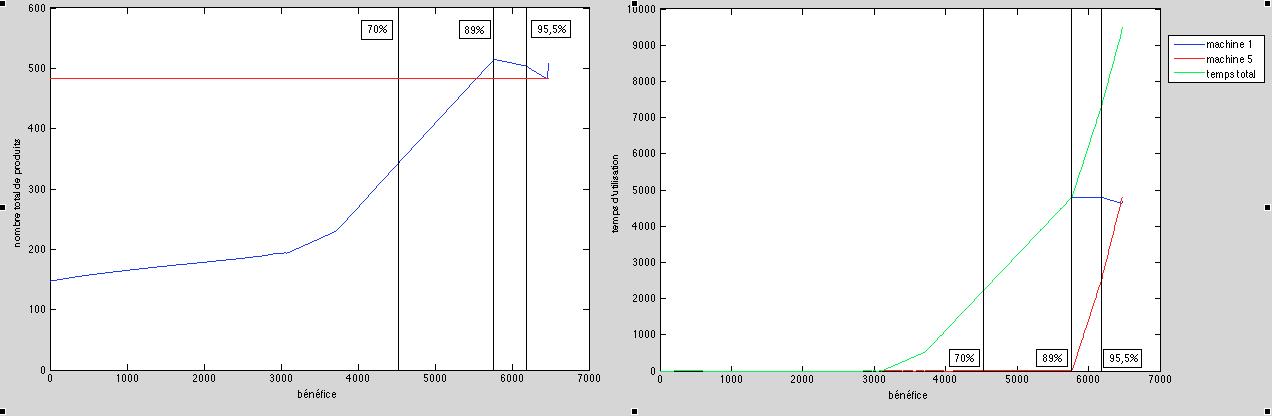
\includegraphics[scale=0.35]{graph_personnel_temps}
        \caption{
            \label{fig_graph_personnel_temps} Legende de l'image (à faire ?).
        }
    \end{center}
\end{figure}

Pour respecter les 70\% du benefice maximum, l’entreprise doit fabriquer un
total de 343.1 produits. Par contre, le deuxième graphique nous montre que la
machine 5 n’est pas du tout utilisée jusqu’aux 89\%. Puisqu’on souhaite
utiliser les deux machines, on choisit un plan de production correspondant à
95,5\% pour raison de changement de la dérivée de la fonction du temps
d’utilisation de la machine 5 à ce point-là. \\

Donc le plan de production est le suivant: \\
$X = (168 168.7394~ 184.0703~ 114.3787~ 36.5623~ 0.0000~ 0.0000)$

\section{Programmation linéaire multicritère}

\section{Analyse multicritère}

\end{document}
